% !TeX spellcheck = pl_PL
\chapter{Wymagania}\label{chap:wymagania}
Aplikacja ma na celu pomóc użytkownikowi zrozumieć i zobrazować działanie algorytmów na sieciach przepływowych. Student, który przygotowuje się do kolokwium z Algorytmów powinien móc utworzyć własną sieć przepływową, prześledzić działanie wybranych algorytmów krok po kroku oraz móc zapisać postęp swojej pracy. Aplikacja ma mieć charakter edukacyjny, umożliwić jak najlepsze przyswojenie omawianych w pracy algorytmów. Wymagania zostały przedstawione w postaci przypadków użycia.
\begin{figure}[H]
	\centering
	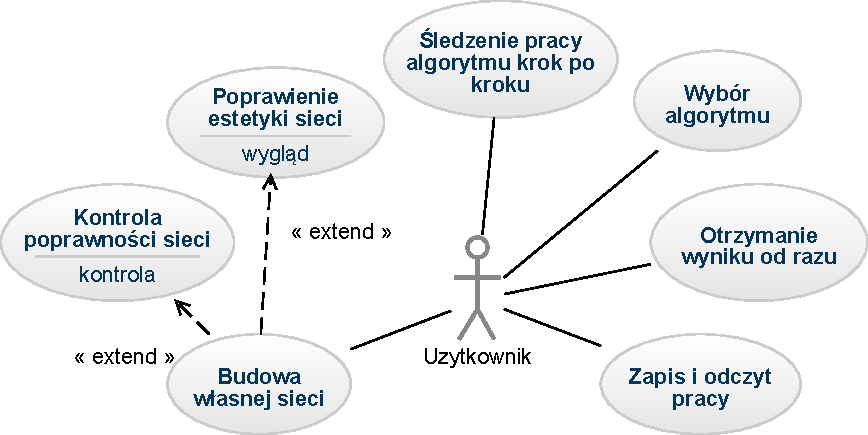
\includegraphics[width=0.8\textwidth]{./img/user_case2}
	\caption{Funkcjonalności wymagane przez potencjalnego użytkownika}
\end{figure}
Ponadto aplikacja powinna zapewnić niezawodność wykonywanych algorytmów. Jeżeli sieci zbudowane przez użytkownika są niepoprawne i nie spełniają założeń, nie powinno dać się wykonywać algorytmów. Użytkownik powinien zostać poinformowany jakie dokładnie błędy popełnił w budowie i co dokładnie należy zrobić by je wyeliminować. Jeżeli siec jest poprawna, algorytm powinien móc dać się wykonać, a jego proces być łatwo kontrolowany przez użytkownika, najlepiej przy pomocy kilku przycisków. Wszystkie zmiany, jakie wprowadził algorytm w danym kroku powinny zostać opisane oraz podświetlone na grafie podglądowym, jeżeli jest to możliwe.
\begin{itemize}
	\item Algorytm Forda-Fulkersona operuje na sieci przepływowej i sieci residualnej, więc wymagane są dwa poglądy zmian,
	\item algorytmy Dinica i MKM ponadto operują na przepływie blokującym, więc wymagane jest utworzenie trzech podglądów zmian.
\end{itemize}
Czas oczekiwania na wykonanie pojedynczego kroku algorytmu powinien być krótki, nieprzekraczający kilku sekund, aby nie nadużywać cierpliwości użytkownika. Aplikacja powinna umożliwiać śledzenie pracy algorytmu zarówno przez małe kroki, jak i skok do końca działania procesu i otrzymania wyniku natychmiastowo, np. w celu porównania go z obliczeniami na kartce.